\documentclass[12pt]{article}
\usepackage{../../eplcrypto}
\usepackage{geometry} % see geometry.pdf on how to lay out the page. There's lots.
\geometry{a4paper} % or letter or a5paper or ... etc
% \geometry{landscape} % rotated page geometry
\usepackage[parfill]{parskip}
% See the ``Article customise'' template for come common customisations
\usepackage{amsmath}
\usepackage{graphicx}
\usepackage{amssymb}
\usepackage{algorithmic}
\usepackage{algorithm}
\title{TP3}

%%% BEGIN DOCUMENT
\begin{document}

\maketitle
\tableofcontents
\newpage

\section{Exercise 1: PRF}
Let $F: \{0,1\}^* \times \{0,1\}^* \rightarrow \{0,1\}^*$ be a length-preserving PRF. Show that no length-presesrving function $F$ can offer the same guarantees in front of an adversary who has an unbounded computational power, that is, for every length-preserving function $F$, there is a (possibly unbounded) disrtinguisher $D$ such that the difference of probabilities in the PRF definition in not negligible.\\

PRF: $\forall$ PPT $D$, $\exists$ negl. $\negl$
\begin{equation*}
|Pr[D^{F_k(\cdot)}=1]-Pr[D^{f(\cdot)}=1]| \le \negl(n)
\end{equation*}
From the look-up table notion, there are $2^{n*2^n}$ functions in $\Func_n$ and selecting $k\leftarrow \zo^n$ and setting the $F_k$ lowers this number to $2^n$. If $D^g$ is unbounded, it can check the output of $g$ for every possible input for all keys $k \in \zo^n$. If it has the same output of $F_k$ for at least one $k$, then it will win.

So as you enumerate for all $k \in \zo^n$ and g is a PRF, we are guaranteed to find the $k$.


\section{Exercise 2: PRP}
Let $F$ be a PRP, and define a fixes-length encryption scheme (Gen,Enc,Dec) as follows: On input $m \in \zo^{n/2}$ and key $k \in \zo^n$, algorithm Enc chooses a random string $r \leftarrow \zo^{n/2}$ of length $n/2$ and computes $c\define F_k(r||m)$. Show how to decrypt, and prove that this scheme is CPA-secure for messages of length $n/2$.\\

\textbf{Decryption:} It is computed by first computing $\FI$ and then outputting $n/2$ LSBs of the result.\\

\textbf{Proof of CPA-security:}\\
Consider an encryption scheme $\Pi'$ that is identical to the one above except that a truly random permutation is used instead of a PRP. Let $\A$ be an adversary and let $q(\cdot)$ be a polynomial upper-bounding the running time of $\A$.

Let $r_c$ denote the random string used to generate the challenge ciphertext $c = F_k(r_c||m)$ There are two cases to consider:
\begin{enumerate}
\item The value $r_c$ is used by the oracle to answer at least one of $\A$'s queries.\\
In this case $\A$ can know which message was encrypted.
\item The value $r_c$ is not used.
\end{enumerate}

Suppose that $\A$ can break the (real, the one with $F_k$) scheme with non-negligible probability $\frac12 + \eta(n)$
\begin{figure}[ht]
    \centering
    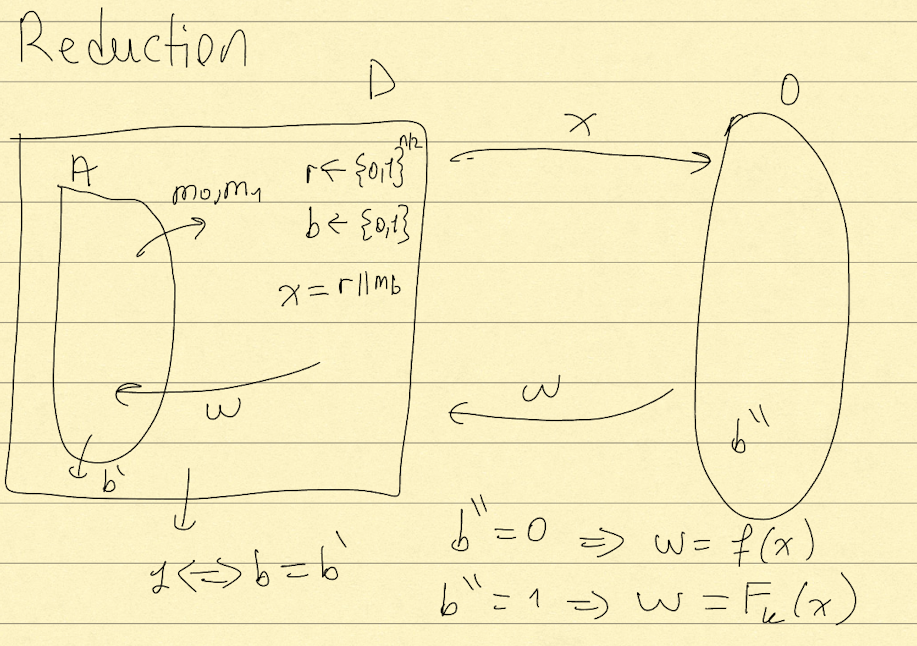
\includegraphics[width=12cm]{figures/f1.png}
\end{figure}

So:
\begin{itemize}
\item If $b''=0$ $Pr[D=1] \le \frac12 + \frac{q(n)}{2^{n/2}}$ : idealized scheme $\Pi'$
\item If $b''=1$ $Pr[D=1] = \frac12 + \eta(n)$ : normal security game with $F_k$
\item $D$ distinguishes with Pr $\ge \eta(n)-\frac{q(n)}{2^n}$
\end{itemize}
\begin{equation*}
|Pr[D^{F_k(\cdot)}(1^n)=1]-Pr[D^{f(\cdot)}(1^n)=1]| \ge \eta(n)-\frac{q(n)}{2^n}
\end{equation*}
Since, $F$ is a PRP, $\eta(n)-\frac{q(n)}{2^n}$ must be negligible, so $\eta(n)$ is negligible. Thus, the difference is negligible.

\section{Exercise 3: CBC}
Consider a stateful variant of CBC-mode encryption where the sender simply increments the $IV$ by 1 each time a message is encrypted (rather than choosing $IV$ at random each time). Show that the resulting scheme is not CPA-secure.

Define $\A$ as follows:
\begin{itemize}
\item Query the Enc oracle with message $m=0^{n-1}||1$, receive a ciphertext $\langle IV, c\rangle $
\item If $IV$ is odd, has the most LSB 1, then output a random bit b
\item If $IV$ is even, the output a pair of messages $m_0, m_1$ where $m_0=^n$ and $m_1$ any other message. Receive in return a challenge ciphertext $\langle IV+1,c' \rangle$
\item If $c'=c$ output $b=0$ else output $b=1$
\end{itemize}

If IV is odd, then $\A$ succeeds exactly half the time (coin toss). For any even IV, it holds that $IV+1=IV \oplus 0^{n-1}||1$ (otherwise it will not work c'=c). Thus for any \textbf{even} IV we have:

\begin{equation*}
c = F_k(IV \xor m) = F_k(IV \xor (0^{n-1}||1) \xor m \xor (0^{n-1}||1)) = F_k((IV+1) \xor m_0)
\end{equation*}

So if $m_0$ is encrypted, then $c'=c$ and $\A$ outputs 0, while if $m_1$ is encrypted then $c'\neq c$ and $\A$ outputs 1.
\begin{equation*}
\frac12 * \frac12 + \frac12 * 1 = \frac34
\end{equation*}

First 1/2 is the probability that IV is odd, then we have 1/2 (second) chance of winning. Third 1/2 is the probability that it is even, then we win every time (1), so it all adds up to probability of winning 3/4 which is not negligible, thus not CPA-secure.
\newpage

\section{Exercise 4: Reduction and/or attacks}


Let $\Pi_1=\langle \Gen^1,\Enc^1,\Dec^1\rangle$ and $\Pi^2=\langle \Gen^2,\Enc^2,\Dec^2\rangle$ be an encryption scheme with $\Enc^1 \colon \K\times \M^1 \mapsto \C^1$ and $\Enc^2 \colon \K\times \M^2 \mapsto \C^2$
\begin{enumerate}
\item If $\C^1 = \M^2$, let $\Pi=\langle \Gen,\Enc,\Dec\rangle$ with
\begin{itemize}
  \item $\Gen\define(\Gen_1,\Gen_2)$ (that is, we obtain two different keys $(k_1,k_2)$
  \item $\Enc_{(k_1,k_2)}(m)\define\Enc_{k_2}^2(\Enc^1_{k_1}(m))$
  \item $\Dec_{(k_1,k_2)}(c)\define\Dec^1_{k_1}(\Dec^2_{k_2}(c))$
\end{itemize}

\begin{enumerate}
\item If $\Pi^1$ is CPA secure, is it $\Pi$ CPA secure?
\item If $\Pi^2$ is CPA secure, is it $\Pi$ CPA secure?
\item If $\Pi$ is CPA secure, is it $\Pi^1$ CPA secure?
\item If $\Pi$ is CPA secure, is it $\Pi^2$ CPA secure?
\end{enumerate}
\item If $\M^1 = \M^2$ and $\C^1 = \C^2$. let $\Pi'=\langle \Gen',\Enc',\Dec'\rangle$ with
\begin{itemize}
  \item $\Gen' \define (\Gen^1,\Gen^2)$ (that is, we obtain two different keys $(k_1,k_2)$
  \item $\Enc'_{(k_1,k_2)}(m) \define (c_1,c_2)$ with $c_1=\Enc^1_{k_1}(m),~c_2=\Enc^2_{k_2}(m))$
  \item $\Dec'_{(k_1,k_2)}(c) \define \Dec_{k_1}(c_1)$ with $c=c_1\|c_2$ ($c_1$ is the first half of $c$)
\end{itemize}

\begin{enumerate}
\item If $\Pi^1$ is CPA secure, is it $\Pi'$ CPA secure?
\item If $\Pi^2$ is CPA secure, is it $\Pi'$ CPA secure?
\item If $\Pi'$ is CPA secure, is it $\Pi^1$ CPA secure?
\item If $\Pi'$ is CPA secure, is it $\Pi^2$ CPA secure?
\end{enumerate}
\end{enumerate}
\newpage
\textbf{1a:}\\
\begin{figure}[h]
    \centering
    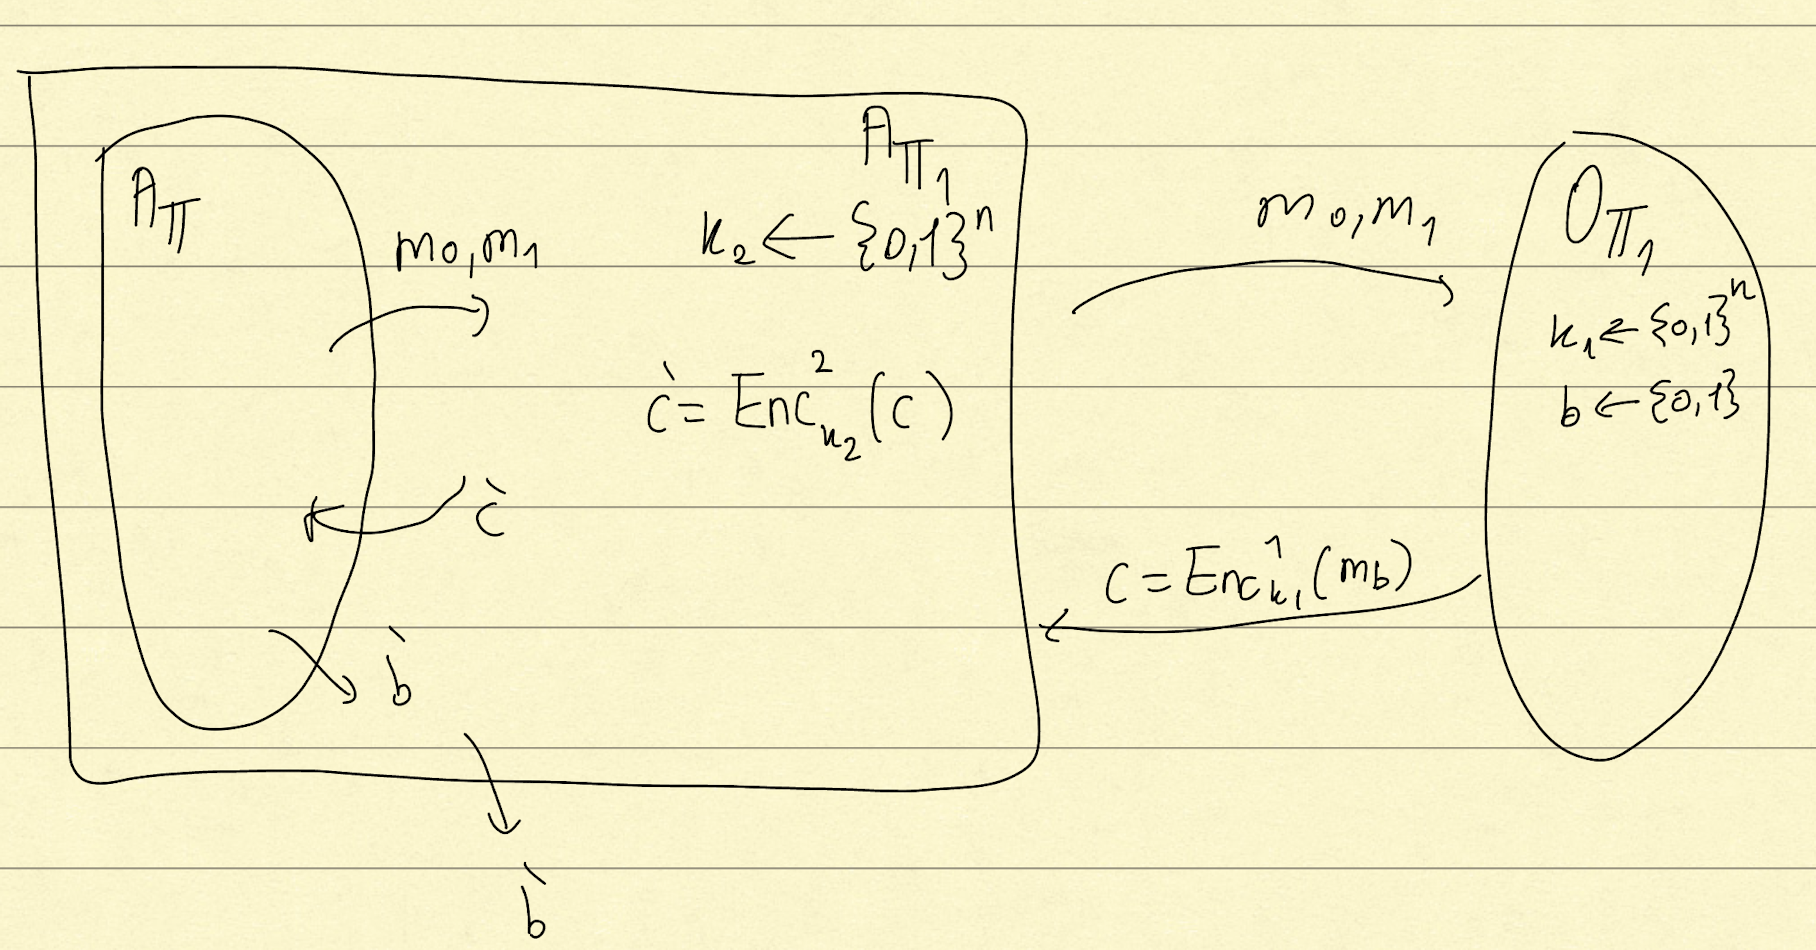
\includegraphics[width=10cm]{figures/f2.png}
\end{figure}

\begin{equation*}
Pr[A_{\Pi^1} \text{ wins}] = \frac12 + \eta(n)
\end{equation*}

Here, $\eta(n)$ is the advantage $A_\Pi$ has against $\Pi$.  If $\Pi^1$ is CPA-secure then $\eta(n)$ is negligible.



\textbf{1b:}\\
\begin{figure}[h]
    \centering
    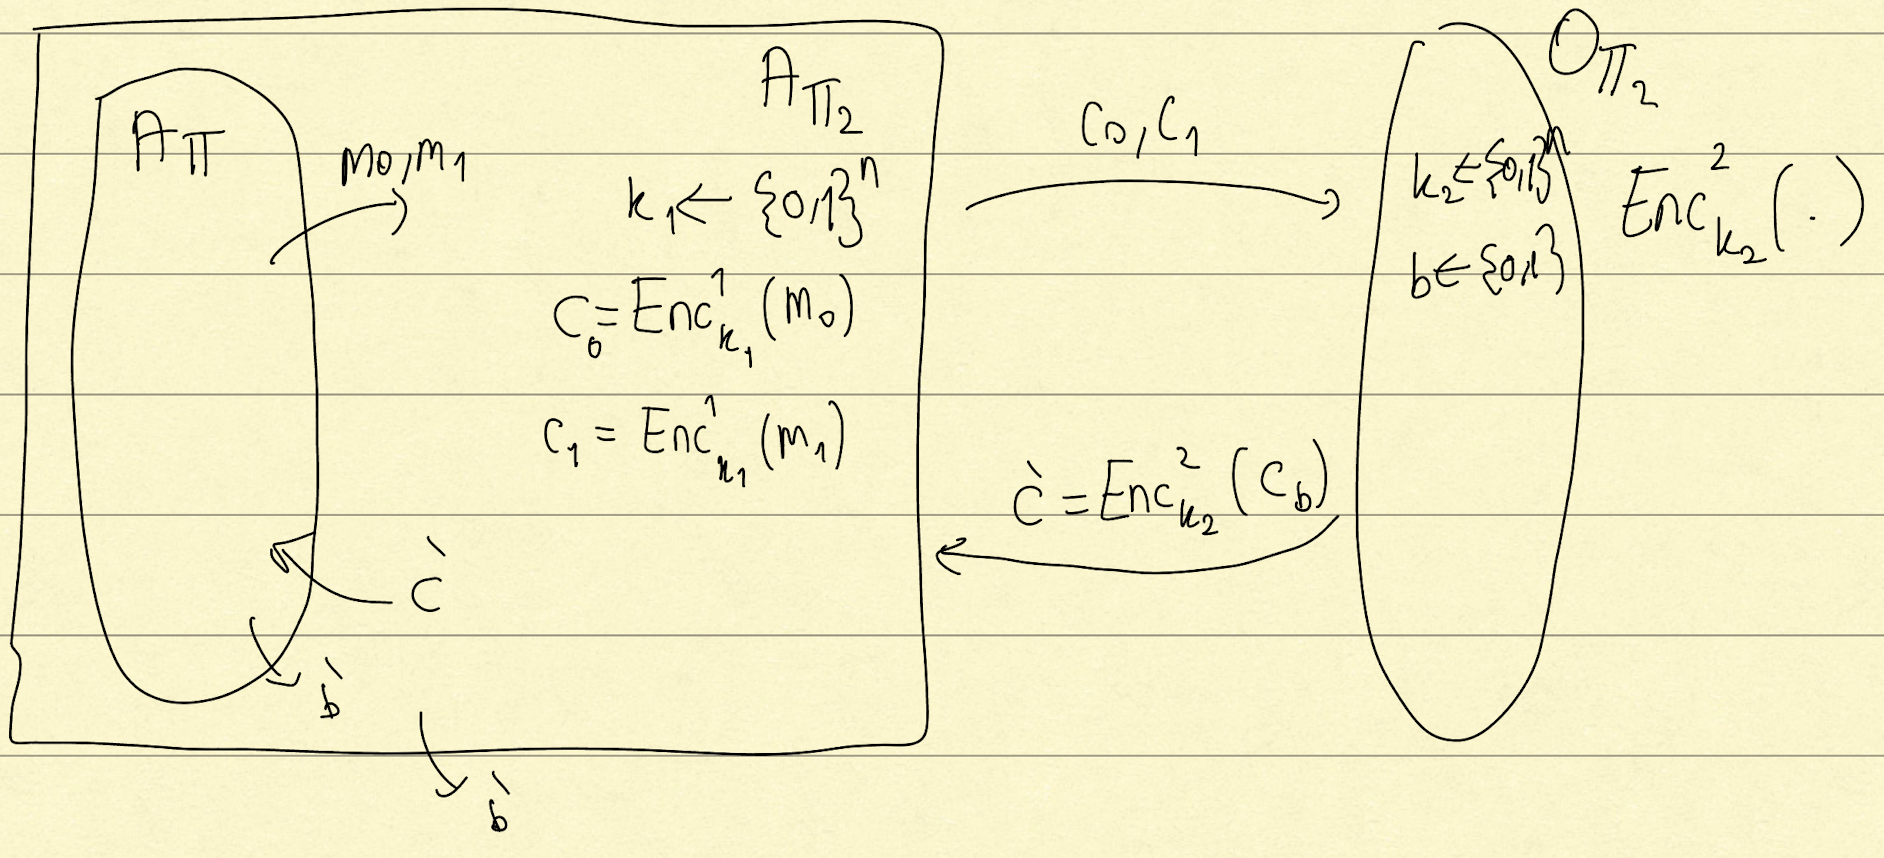
\includegraphics[width=10cm]{figures/f3.png}
\end{figure}

\begin{equation*}
Pr[A_{\Pi^2} \text{ wins}] = \frac12 + \eta(n)
\end{equation*}

Here, $\eta(n)$ is the advantage $A_\Pi$ has against $\Pi$. If $\Pi^2$ is CPA-secure then $\eta(n)$ is negligible.

\textbf{1c:}\\
We cannot say for sure, since $\Pi$ can encrypt like $Enc_{k_1}^1(m)=m$ and let's say $\Pi^2$ is still CPA-secure and $\Pi$ would still work. So, we cannot build an adversary that can use $\A_{\Pi^1}$ to break $\Pi$.\\

\textbf{1d:}\\
Same as above, now $\Pi^2$ might be doing $Enc_{k_2}^2(m)=m$ and $\Pi^1$ be CPA-secure and $\Pi$ would still work.So, we cannot build an adversary that can use $\A_{\Pi^2}$ to break $\Pi$.


\textbf{2a and 2b:}\\
For $\Pi'$ to be secure both $\Pi^1$ and $\Pi^2$ need to be CPA-secure. If one of them are identity encryption then the adversary just needs to look at half of the cipher text and check if one of them correspond to any of challenge messages and output the correct bit.

\textbf{2c:}\\
\
Can we use $\Pi^1$ to break $\Pi'$?
\begin{figure}[h]
    \centering
    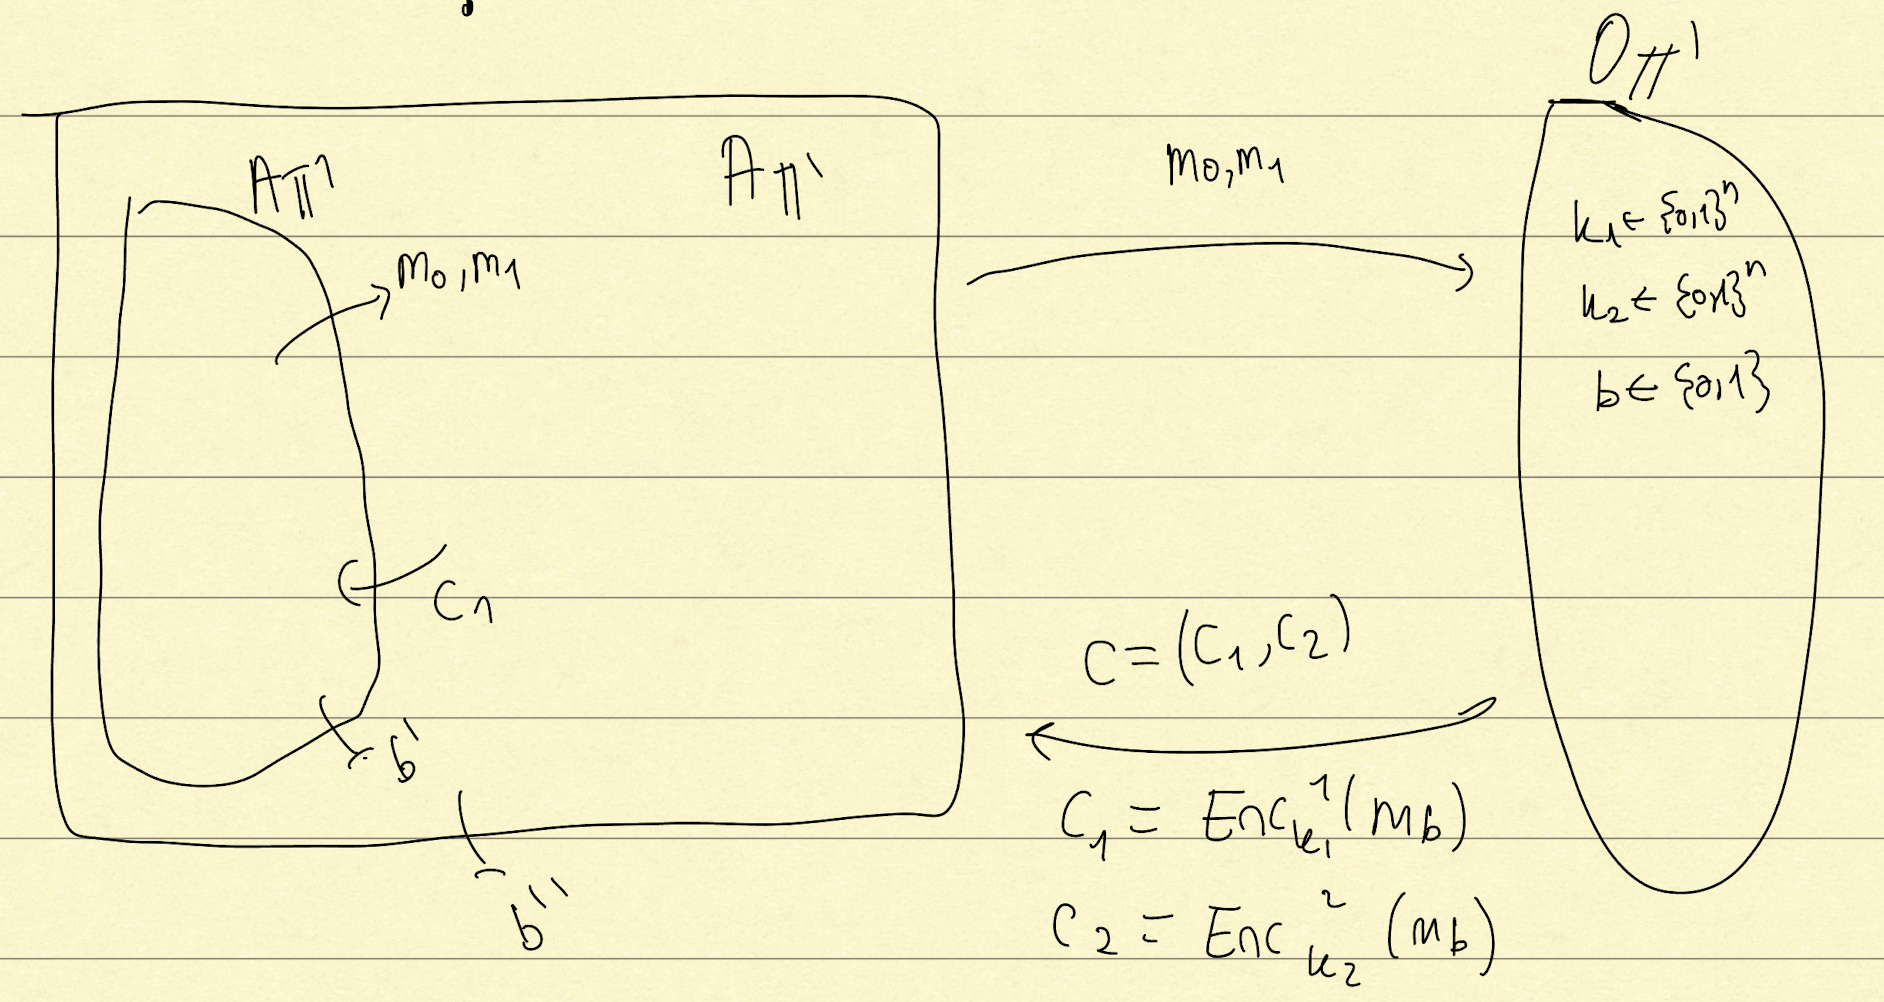
\includegraphics[width=10cm]{figures/f4.png}
\end{figure}

\[ \Pr[\PrivKcpa[\A_{\Pi'}, \Pi'](n)=1] = \Pr[b''=b] = \Pr[b'=b] = \Pr[\PrivKcpa[\A_{\Pi^1}, \Pi^1](n)=1] = \frac12 + \eta(n) \]\\
where $\eta(n)$ is the advantage of $\A_{\Pi^1}$ against $\Pi^1$. If  $\Pi'$ is CPA-secure then $\eta(n)$ is negligible.

\textbf{2d:}\\
Same reduction as above but now $\A_{\Pi^2}$ is used as subroutine and $c_2$ is returned to it.

\end{document}